\chapter{Vorgehensmodell}

Nachdem im letzten Kapitel der aktuelle Aufbau der Payment-Anwendungen, sowie die durch die monolithische Struktur hervorgebrachten Probleme, erläutert wurden, werde ich im Folgenden beschreiben wie ich vorgehen werde um den Problemfokus der Startzeit zu untersuchen.

\section{Anforderungen an Daten zur Messung des Startup-Verhaltens von Containern}
\begin{itemize}
  \item Problem reduzieren
  \item Messkriterien festlegen
  \item Quellen finden
  \item hier nur theoretisch schwafeln über einen kriterienkatalog und die möglichen „Messwerte“, die man ggf. braucht -> in Kap. 5 dann den Kriterienkatalog konkret aufstellen
\end{itemize}

Der Fokus des Projekts liegt allerdings auf der Ermittlung der Cloudfähigkeit der unterschiedlichen System-Komponenten. Um dies festzustellen, muss im Vorwege eine Klassifizierung der Anforderungen stattfinden um festzustellen welche Messdaten für dieses Projekt überhaupt von Relevanz sind. Hierfür hat die ISO bereits einen ausführlichen Kriterienkatalog aufgestellt(siehe ISO/IEC 25010:2011 \cite{iso25010}, fig. \ref{fig:iso25010}). Die ISO 25010 besteht aus acht Hauptkategorien und 31 Unterkriterien, wobei lediglich die erste Hauptkategorie der "\emph{Funktionalität}" dabei als \emph{funktionale Qualitätseigenschaft} (engl. "\emph{functional requirement}") auftritt. Die restlichen Hauptkriterien lassen sich der Kategorie der \emph{Non-Functional requirements} zuordnen. Diese Unterscheidungen dienen als eine erste Abstraktionsschicht. Functional requirements beschreiben hierbei die Korrektheit des Produktes \cite{continuous-delivery}. "Sie spezifizieren die Funktion, die ein System oder Systemkomponente erfüllen muss" \cite{eide-requirements}. So lässt sich feststellen ob die Applikation den inhaltlichen Ansprüchen, sowohl aus technischer als auch aus Unternehmenssicht, genügen. Hierbei wird auf eine Vielzahl unterschiedlicher Tests zurückgegriffen, welche sich auf breit gefächerte Abstraktionstiefen etc. beziehen lassen (siehe \ref{fig:testing-quad}). Je nach Teilbereich lassen sich hierbei einzelne Gebiete automatisiert oder mittels anderweitiger Werkzeuge testen. Diese Tests sind in einem System in Produktion unabdingbar, für die Messdatenerhebung zur Beurteilung der Cloudfähigkeit allerdings vernachlässigbar. 

Zur Eingrenzung der Anforderungen an die Messdaten sind viel mehr die \emph{Non-Functional Requirements} von Bedeutung. Sie beschreiben nicht \emph{was} vom System geleistet werden muss, sondern \emph{wie} dies geschehen soll, deshalt werden die Kriterien unter anderem auch \emph{system-quality attributes} genannt. Im Folgenden werden die für das Projekt relevanten Kriterien einmal zusammengefasst dargestellt.

\begin{figure}[h!]
	\centering
	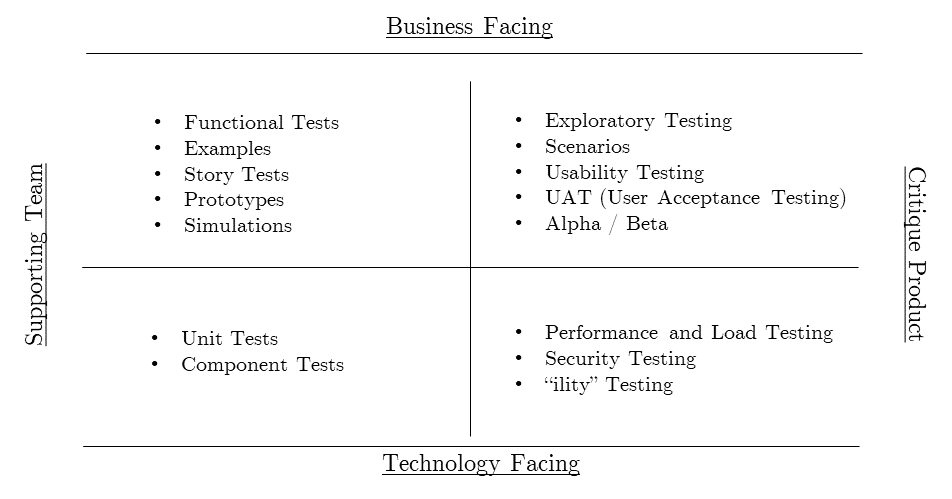
\includegraphics[width=\linewidth]{kapitel/vorgehensmodell/_img/agile-testing-quadrants}
	\caption[Agile Testing Quadrants]{Agile Testing Quadrants}
	\label{fig:testing-quad}
\end{figure}

\begin{figure}[h!]
	\centering
	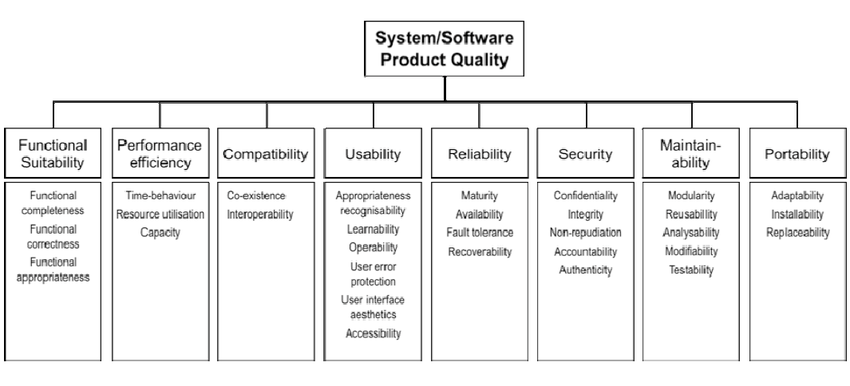
\includegraphics[width=\linewidth]{kapitel/vorgehensmodell/_img/iso25010}
	\caption[iso25010]{ISO 25010}
	\label{fig:iso25010}
\end{figure}



\subsubsection{Leistungsfähigkeit}
% https://www.dotnetcurry.com/project-management/1462/non-functional-requirements-nfrs
\begin{itemize}
  \item "Performance of a product or an app defines how a product/app is performing or behaving as compared to its expected behavior"
  \item Reaktionszeiten, wie schnell ist app wenn User interagiert
  \begin{itemize}
    \item eng verwand \emph{Latenz / Delay}, wie lange darf ein User max. warten müssen (Threshold ist die Reaktionszeit)
    \item typischerweise pro Screen gesetzt, kann aber auch auf die Masse bezogen werden (bspw. 80 Prozent der Interaktionen haben eine Reaktionszeit von max. 3 Sekunden)
  \end{itemize}
  \item Durchsatz: Anzahl der Daten, welche die Applikation handlen kann
  \begin{itemize}
    \item kann sich sowohl auf Benutzeranfragen, db Anfragen, API calls etc. beziehen
    \item Durchsatzziele als Teil der Anforderungsanalyse
    \item werden mittels Performance / Load Testing validiert
  \end{itemize}
  \item tools wie gatling / Jmeter fuer diesen Usecase unpassend, da nicht die Api Anfrage sondern nur die Hochfahrzeit gemessen werden soll
  \item 
\end{itemize}

\emph{"Performance of a product or an app defines how a product/app is performing or behaving as compared to its expected behavior" \cite{nfr-dotnetcurry}}. Die Leistungsfähigkeit einer Anwendung setzt sich aus den Punkten \emph{Zeitverhalten}, \emph{Ressourcennutzung} sowie \emph{Kapazität} zusammen. Das Zeitverhalten wird vorallem durch die Reaktionszeit der Applikation geprägt. Es wird gemessen wie schnell auf Benutzereingaben eingegangen werden kann. Eng verwand ist hierbei auch der Begriff der \emph{Latenzzeit}, da dieser beschreibt wie lange eine Beantwortung der Anfrage in Praxis letztendlich dauert. Die Reaktionszeit dient hierbei als ein Threshold der nicht überschritten werden sollte. Typischerweise wird die Reaktionszeit pro Client festgelegt, es ist jedoch auch möglich, dies für eine Menge von mehreren Clients festzulegen. Ein Beispiel wäre festzulegen, dass ein bestimmter Anteil der Interaktionen eine maximale Reaktionszeit von \emph{n} Sekunden besitzt. Aber auch das zweite Unterkriterium der \emph{Resourcennutzung} darf nicht vernachlässigt werden, so dürfen zum Beispiel bestimmte Kommunikationsschnittstellen nicht überlastet werden oder diverse Connectionspools nicht überlaufen, da es sonst zu Timeouts kommen könnte. Die Kapazität beschreibt zum Beispiel die Anzahl von möglichen parallelen Anfragen oder wie viele Nachrichten übermittelt beziehungsweise vom System gespeichert werden können. Ein weiterer Unterpunkt, welchen man der Leistungsfähigkeit zuschreiben kann, ist der des \emph{Durchsatzes}. Dieser Begriff wird in der ISO Norm allerdings nicht erwähnt. Im Idealfall möchte man nicht nur feststellen, wie lange Nachrichten verarbeitet werden, sondern auch wie viele im Schnitt verarbeitet werden können. Der Datendurchsatz ist also durchaus auch von größerem Interesse und sollte definitiv gemessen werden. Die verarbeiteten Daten können sich hierbei auch auf verschiedenes beziehen. Es können zum Beispiel die Anzahl von Anfragen an eine API sowie deren Rückmeldung sein, oder diverse Messages an Broker, welche durch das System gereicht werden. Es kann sich aber auch ganz banal auf die Anzahl der Datenbankanfragen etc. beziehen. Diese Art der Performanz wird in der Regel mittels spezieller Tools, wie zum Beispiel "\emph{Gatling}" oder  "\emph{JMeter}" in sogenannten \emph{Performance} oder auch \emph{Load Tests} validiert. Alles in allem stellt die Leistungsfähigkeit mit ihren Subkategorien eine der wohl wichtigsten Kriterien dar. 


\subsubsection{Skalierbarkeit}
\paragraph{Hardware}
\begin{itemize}
  \item je nach Anforderungen hoch oder herunterfahren
  \item \emph{concurrent users} : Wie viele Benutzer verwenden zeitgleich die Applikation. I.d.R. 20 - 30 Prozent der Userbase. Kann auf 100 Prozent bei besonderem Event hochgehen
  \item Zeitfaktor nicht vergessen, Applikation Skalierung sollte auch zeitlich gesteuert werden
  \item \emph{vertikale Skalierung / scaling up} : Mehr CPUs / RAM fuer existierende Infrastruktur
  \item \emph{hori Skalierung / scaling out} : mehr Server
  \item vielleicht Bild einfuegen scale out vs scale up
  \item cloud provider verwenden generell scale out
\end{itemize}

\paragraph{Software}
\begin{itemize}
  \item Bsp. Ladezeiten einer single page application zu hoch (z.B. Laden von Daten aus DB), scale out bringt hierbei nichts...
  \item Performanz sollte von Anfang an bedacht werden
  \item Frameworks sollten auf multithreading etc. ausgelegt sein, vor Verwendung einmal überprüfen
  \item Bottlenecks früh bestimmen, Legacy Libs eventuell austauschen
  \item Load Balancer sollte in irgendeiner Art vorhanden sein um Hardware Skalierung mit Software in Verbindung zu bringen
  \item Ohne Session Management ist die Performance schlecht, gilt es ebenfalls im Vorwege zu prüfen
\end{itemize}
Ein weiteres wichtiges Kriterium welches allerdings nicht direkt in der ISO 25010 Norm auftritt, ist die Skalierbarkeit des Systems. Bei der Beurteilung kommt gilt es in erster Linie zwischen dem Skalieren der \emph{Hardware} sowie der \emph{Software} zu unterscheiden \cite{nfr-dotnetcurry}. Die Hardwareskalierung könnte man grob dem Unterkreterium "\emph{Ressourcennutzung}" zuordnen. Denn in einer modernen containerisierten Cloud-Umgebung soll es möglich sein, die einzelnen Komponenten nicht nur auf einem Gerät beliebig zu skalieren, sondern falls die aktuelle Hardware an ihre Kapaziätsgrenzen stößt auch noch weitere Hardwarekomponenten hinzuziehen können. Inwiefern dies automatisiert oder manuell geschieht lässt sich nur fallabhängig bestimmen, es sollte jedoch evaluiert werden ob dies überhaupt generell möglich ist. Metriken zum Ermitteln des Skalierungszeitpunkt könnten zum Beispiel die Anzahl der parallel arbeiten Benutzer der Applikation (engl. "\emph{concurrent users}"), die Latenzzeit oder die CPU Auslastung der beteiligten Maschinen sein. Es ist allerdings auch wichtig, dass eine Applikation nicht nur von aktiv eingehenden Ereignissen skaliert wird, sondern auch ein Zeitverhalten mit sich bringt und sich selbstständig zeitabhängig skalieren kann. Dies macht den Skalierungsprozess robuster, da sich die Komponente dadurch wieder etwas von seiner Umwelt abgrenzen kann (welche in der Regel durchaus fehlerbehaftet sein kann). Bei der Hardwareskalierung gibt es zwei wesentliche Arten, die \emph{vertikale} und die \emph{horizontale Skalierung}. Der Begriff der \emph{vertikalen Skalierung} (auch \emph{scale up} Skalierung) beschreibt das modifizieren der Servereigenen Resourcen. Dazu können zum Beispiel die Anzahl der CPU Kerne oder der verfügbare Speicher gehören. Dieses Verfahren wird in monolithischen Strukturen mit älteren Systemen verwendet, die nicht darauf ausgelegt sind, sich auf mehrere Server zu verteilen. Dagegen steht der Begriff der \emph{horizontalen Skalierung} (auch \emph{scale out} Skalierung), welcher gerade dieses Auslagern bestimmter Komponenten beziehungsweise Prozessinstanzen auf neue Hardware beschreibt. Dieser Ansatz wird in der Cloud-Technologie verfolgt und nicht nur auf \emph{on premise} \todo{Footnote on premise}, sondern auch von den großen \emph{public cloud vendorn} \todo{footnote public cloud vendor} wie zum Beispiel Amazon AWS oder Microsoft Azure, verwendet.

Dennoch muss die Software auf eine Skalierung der Hardware ausgelegt sein. Manche Probleme lassen sich mit mehr Rechenperformance nicht lösen, wenn zum Beispiel die Ladezeiten bestimmter Kommunikationsschnittstellen einen Bottleneck darstellen. Alter Legacy Code könnte ebenfalls Performanceeinbußen darstellen und ohne ein vernünftiges Session Management bringt auch das Skalieren der Hardware nichts. Diese Grundfunktionalitäten werden heutzutage jedoch von fast allen Frameworks standardmäßig mitgeliefert. Dennoch gilt es dies im Vorwege noch einmal zu validieren. 


\subsubsection{Kompatabilität}
Dieses Hauptkriterium beschreibt, wie nebenläufig das System im Endeffekt ist. Ist es möglich, dass mehrere Komponenten gleichzeitig arbeiten können, ohne sich gegenseitig zu behindern? Gerade in einer Containerisierten Umgebung ist dies von fundamentaler Wichtigkeit. Der Unterbegriff \emph{Ko-Existenz} beschreibt gerade dieses Verhalten. Der zweite Unterbegriff der "\emph{Interoperabilität}" beschreibt inwiefern die verschiedenen Komponenten in der Lage sind Daten untereinander auszutauschen. Wie genau dieser Datenaustausch aussieht kann sich von System zu System unterscheiden. Zusammenfassend lässt sich sagen, dass diese Kriterien in einer cloudbasierten Anwendung zwar gelten müssen, sie allerdings dennoch derartig abstrakt gehalten sind, dass es schwieriger ist hier messbare Metriken zu generieren. Entweder das System funktioniert oder es ist fehlerhaft, einen messbaren Mittelweg gibt es nicht direkt.

\subsubsection{Zuverlässigkeit}
% https://www.dotnetcurry.com/project-management/1462/non-functional-requirements-nfrs
\begin{itemize}
  \item High Availability
  \item Angabe wie lange app garantiert laeuft (bspw. Prozentangabe pro Jahr)
  \item Design for failure: Komponenten darauf ausgelegt, dass Ausfall einzelner Komponenten zu keinem Systemausfall fuehrt
  \item accessibility: app ist nicht für die Allgemeinheit konzipiert worden
\end{itemize}

Das Hauptkriterium der \emph{Zuverlässigkeit} beschreibt die Angabe wie lange eine Applikation garantiert läuft. Dies kann auf verschiedene Weisen festgehalten werden, eine typische wäre zum Beispiel den Anteil der Tage im Jahr, Tage pro Monat, oder Stunden am Tag die ein Service ansprechbar ist. Allgemein lässt sich diese Angabe als Metrik der \emph{Verfügbarkeit} charakterisieren. In einer Containerisierten Umgebung kommt es immer wieder zu Ausfällen einzelner Systeme, was es bei diesem Punkt besonders zu beachten gilt. Das Gesamtsystem soll hiervon jedoch unberührt bleiben. Dieses Prinzip wird in heutigen Systeme auch "\emph{Design for failure}" genannt. Das Hauptkriterium setzt sich aus unter anderem aus dem Unterkriterium der \emph{Reife} zusammen. Hierbei sind diejenigen Anforderungen gemeint, welche in einer normalen Prozessabarbeitungsphase ohne besondere Ereignisse hinsichtlich zum Beispiel der Anzahl der zu verarbeitenden Nachrichten, oder der Komplexität der zu bewältigenden Aufgaben, gelten müssen. Auch eine gewisse \emph{Fehlertoleranz} wird vom System erwartet. Um dies zu testen genügt es bereits dokumentierte allerdings fehlerbehaftete Benutzereingaben in einer Testumgebung zu tätigen und das Systemverhalten zu analysieren. Eine standardisierte Metrik gibt es auch nicht. Das letzte Unterkriterium der \emph{Zuverlässigkeit} ist die \emph{Wiederherstellbarkeit} nach einem beschriebenen Fehlerfall, falls es doch einmal zu einem Ausfall einzelner Komponenten kommen sollte. Generell gilt, auch dieses Hauptkriterium gibt Aufschluss über die Eignung gewisser technologischer Ansätze zum Arbeiten als Cloudkomponente, dennoch beschreibt sie die relevanten Umstände in manchen Teilen zu abstrakt als das man dort genaue Metriken ermitteln könnte. Im nächsten Kapitel wird festgehalten welche Metriken dennoch relevant erscheinen. \todo{Ref einbinden bzw. schauen ob überhaupt aufgenommen...}

\subsubsection{irrelevante Themenfelder}
\begin{itemize}
  \item Security (Injection, Broken Authentication, Cross Site Scripting etc.)
  \item Nutzbarkeit (Benutzerfreundlichkeit, Browser Kompatabilität, Internationalisierung - Eingabesprachen)
\end{itemize}

Weitere Hauptkriterien der ISO Norm betreffen die \emph{Nutzbarkeit}, sowie die \emph{Sicherheit} der Anwendung. Da der Fokus des Projekts aber darin liegt die Skalierbarkeit sowie die Performance des Systems zu testen, können all diese Punkte jedoch vernachlässigt werden. Die Themengebiete der \emph{Wartbarkeit} sowie der \emph{Übertragbarkeit} sind in einer containerisierten Plattform zwar ebenfalls unabdingbar, sind allerdings derartig abstrakt gehalt, dass es den Rahmen dieser Thesis sprengen würde ebenfalls näher auf diese einzugehen. 

\section{Anforderungen an Prototypen}
\begin{itemize}
  \item einmal als spring boot und einer weiteren variante mit einer cloud-native technologie -> hier wurde vorgegeben mit serverless zu arbeiten.
\end{itemize}

Bei diesem Projekt sollen sowohl Orchestrierungsplattformen als auch die tatsächlich laufende Runtime Umgebung beziehungsweise ein entsprechendes Framework verglichen werden. 

Hinsichtlich der Skalierung soll es beispielsweise möglich sein, anhand festgelegter Regeln eine automatische \emph{horizontale} Skalierung stattfinden. Dieses Verhalten soll sowohl in hinterlegten Datensätzen als auch mittels eines eigens dafür eingerichteten Dashboards nachvollziehbar dargestellt werden. Auf welche Technologien sowohl bei der Skalierung sowie der Darstellung beziehungsweise Berechnung der Metriken zurückgegriffen wird, wird vom Arbeitgeber nicht vorgegeben. Lediglich hinsichtlich der Komponenten zur Verarbeitung der Business Logik wurde eine Vorauswahl getroffen. Wie bereits angedeutet, wird die aktuell laufende Java Enterprise Applikation mit dem moderneren Spring Boot Framework ersetzt um einen aktuelleren Vergleichspunkt in puncto kompilierbare Applikation getroffen. Um einen sinnvollen Vergleichspunkt anzusetzen, wird dem eine cloud-native Technologie gegenübergestellt. "Cloud Native beschreibt einen Software-Entwicklungs-Ansatz, bei dem Applikationen von Anfang an für den Einsatz in der Cloud konzipiert werden. Das Ergebnis sind Native-Cloud-Applikationen (NCAs), die die Stärken der Cloud-Computing-Architektur vollständig zu nutzen wissen." \cite{cn-def} Mit dieser doch relativ abstrakt gehaltenen Definition, sind hinsichtlich der verarbeitenden Komponenten allerdings in erster Linie die modernen Skript-Frameworks gemeint. Hierbei gibt es mehrere Alternativen, wo es seitens des Arbeitgebers allerdings ebenfalls keinerlei genaue Vorgaben hinsichtlich des spezifischen Frameworks / Technologie gibt.

\subsection{Festlegung fiktiver Workflow}
\label{ss:fiktiverWorkflow}
Da der Fokus auf der Untersuchung der Startupzeit der Komponenten liegt, wird lediglich eine minimale beispielhafte Implementierung erfolgen, welche die Arbeitsschritte der eigentlichen Applikation in vereinfacht darstellen soll. Es soll im Rahmen dieser Arbeit eher als ein \emph{proof of concept} gelten. Allerdings werden im System konkrete Nachrichten im XML Format vermittelt, welche einer XSD-Spezifikation folgen wie sie im realen Umfeld ebenfalls genutzt wird. 

\todo{Auszug aus XML einbinden???}

Sobald eine neue Nachricht eingetroffen ist, soll drei Arbeitsschritte ausgeführt werden:

\begin{enumerate}

  \item Es soll geprüft werden, ob das eingegangene XML der XSD-Spezifikation folgt oder nicht. Wenn dies nicht der Fall sein sollte, wird die Nachricht zwar derartig acknowledged, dass sie zwar aus der Eingangsqueue im Message Broker enfernt wird, allerdings bei der Verarbeitung ignoriert wird.

  \item Falls es sich um valides XML handelt, wird ein Feld aus dem XML-Inhalt ausgelesen.

  \item in einem letzten Schritt wird dieses Element in eine Datenbank geschrieben damit auch eine Persistenz-Operation in die Verarbeitungszeit einfließt.

\end{enumerate}

\subsection{Spring Boot}
Wie bereits angedeutet, wird die aktuell laufende Java Enterprise Applikation mit dem moderneren Spring Boot Framework ersetzt um einen aktuelleren Vergleichspunkt in puncto kompilierbare Applikation getroffen. Um einen sinnvollen Vergleichspunkt anzusetzen, wird dem eine cloud-native Technologie gegenübergestellt. Die Komponenten sollen beide die beschriebenen Arbeitsschritte abbilden.

\subsection{Serverless}
\begin{itemize}
  \item  4.2.2 spring boot 4.2.3 serverless -> so bekommt der prof schon beim draufgucken auf das inhaltsverzeichnis die story mit….
\end{itemize}
Um der kompilierten Spring Boot Anwendung eine Technologie ein auf skalierbare Komponenten ausgelegt Technologie gegenüberzustellen, wird hierbei auf eine cloud-native Technologie gesetzt. "Cloud Native beschreibt einen Software-Entwicklungs-Ansatz, bei dem Applikationen von Anfang an für den Einsatz in der Cloud konzipiert werden. Das Ergebnis sind Native-Cloud-Applikationen (NCAs), die die Stärken der Cloud-Computing-Architektur vollständig zu nutzen wissen." \cite{cn-def} Mit dieser doch relativ abstrakt gehaltenen Definition, sind hinsichtlich der verarbeitenden Komponenten allerdings in erster Linie die modernen Skript-Frameworks gemeint. Hierbei gibt es mehrere Alternativen, wo es seitens des Arbeitgebers allerdings ebenfalls keinerlei genaue Vorgaben hinsichtlich des spezifischen Frameworks / Technologie gibt.

\section{Anfoderungen an Containerisierungsplattform / Orchestrierungsplattform}
Es gibt zwar diverse Containerisierungsplattformen \todo{continuous delivery zitieren und aufzaehlen} dennoch hat sich vorallem die Technologie "\emph{Docker}" durchgesetzt, die Vorteile und generelle Funktionsweise wurden bereits relativ ausführlich erläutert. Deshalb soll diese auch im Prototypen Verwendung finden. Hinsichtlich der Orchestrierungsplattform (welche auch als \emph{Clustering Werkzeug} dient) werden folgende Anforderungen formuliert. 

\section{Anforderungen an Lasttest}
Es soll möglich sein, das System in einem einheitlichen Format mit Nachrichten zu versorgen. Hierfür benötigt man eine Benutzerschnittstelle, die es ermöglicht dem Benutzer möglichst aussagekräftige Befehle ohne allzu viel Konfigurationsaufwand zur Verfügung zu stellen. Diese Befehle müssen anschließend intern wiederum in detailierte Nachrichten umgewandelt werden, welche durch das System gereicht werden können. Hierfür gibt es die Möglichkeit einer Benutzeroberfläche im Browser oder der Festlegung eines Formats im Body einer Http-Anfrage an eine REST-Api. Eine Skalierung auf meherere Systeme sollte zwar einmal testweise erfolgen, für die Generierung der Metriken ist dies allerdings eher hinderlich, da es die Ergebnisse verfälschen könnte. Da es dem Design der Orchestrierungsplattform geschuldet ist, dass der Anwender wenig Einfluss auf die Resourcenzuteilung hat, kann es passieren, dass eine leistungsschwächere Maschine deutlich mehr Initialisierungsanfragen zugewiesen bekommt. Dies könnte man zwar dadurch umgehen, dass man zwei exakt gleichbestückte Server für den Lastentest verwendet. Hierbei würden im Nachhinein allerdings die gleichen Ergebnisse erlangt werden, wie bei Testlauf auf einer Maschine.

\section{Anforderungen Visualiserung und Monitoring zur Unterstützung der Auswertung}
Es muss möglich sein, Metriken automatisch vom System generiern zu lassne. Dazu müssen die Datensätze persistent hinterlegt werden, um auch im Nachhinein nachvollziehen zu können wie die Metriken entstanden sind. Außerdem muss eine grafische Aufarbeitung erfolgen. Diese Visualierung soll in Echtzeit oder einem zeitlich festgelegten Intervall aktualisiert werden können. Bezüglich des genauen Werkzeugs werden keinerlei Vorgaben gegeben, um dem Benuzter jedoch jeglichen Installationsaufwand zu ersparen wäre eine webbasierte Darstellung sicherlich von Vorteil.
